%%---------------------------------------------------------------------------%%
%% Shift Roadmap Presentation
%%---------------------------------------------------------------------------%%

\documentclass{beamer}
\usefonttheme[onlymath]{serif}
\usepackage{colortbl}
\usepackage{longtable,ltcaption,array}
%% The amssymb package provides various useful mathematical symbols
\usepackage{amssymb}
%% The amsthm package provides extended theorem environments
\usepackage{amsthm} \usepackage{amsmath} \usepackage{tmadd,tmath}
\usepackage{booktabs}
\usepackage{multirow}
\usepackage{caption}
\usepackage[labelformat=empty]{subcaption}
\usepackage{tabularx}

%%---------------------------------------------------------------------------%%
%% THEME SETUP

\usetheme{CambridgeUS}
\usecolortheme{spruce}

%%---------------------------------------------------------------------------%%
%% SETUP STUFF
%%---------------------------------------------------------------------------%%

\logo{
\includegraphics[width=2cm]{new_logo}}

\setbeamercolor{item}{fg=MSUgreen}
\setbeamertemplate{headline}{}
\setbeamertemplate{navigation symbols}{}

\newlength{\DUtablewidth} % internal use in tables

%%---------------------------------------------------------------------------%%
%% MATH STUFF
%%---------------------------------------------------------------------------%%

\newcommand{\Pn}{\textit{P}$\negthinspace_N$}
\newcommand{\SPn}{\textit{SP}$\negthinspace_N$}

\newcommand{\vOmega}{\ensuremath{\ve{\Omega}}}
\newcommand{\hOmega}{\ensuremath{\hat{\ve{\Omega}}}}

\newcommand{\sigs}{\ensuremath{\sigma_{\text{s}}}}
\newcommand{\sigf}{\ensuremath{\sigma_{\text{f}}}}
\newcommand{\sigsm}{\ensuremath{\sigma_{\text{s}m}}}
\newcommand{\sigsn}{\ensuremath{\sigma_{\text{s}n}}}

\newcommand{\phig}{\ensuremath{\Phi}}
\newcommand{\Sigmag}{\ensuremath{\mathbf{\Sigma}}}
\newcommand{\Dg}{\ensuremath{\mathbb{D}}}
\newcommand{\Fg}{\ensuremath{\mathbb{F}}}
\newcommand{\Qg}{\ensuremath{\mathbb{Q}}}
\newcommand{\ug}{\ensuremath{\mathbb{U}}}
\newcommand{\Ag}{\ensuremath{\mathbb{A}}}
\newcommand{\Bg}{\ensuremath{\mathbb{B}}}
\newcommand{\Cg}{\ensuremath{\mathbb{C}}}
\newcommand{\Jg}{\ensuremath{\mathbb{J}}}
\newcommand{\sg}{\ensuremath{\mathbb{S}}}

\newcommand{\aphig}{\ensuremath{\Phi^{\dagger}}}
\newcommand{\aSigmag}{\ensuremath{\mathbf{\Sigma}^{\dagger}}}

\newcommand{\apsi}[1]{\ensuremath{\psi^{\dagger\,#1}}}
\newcommand{\aphi}[1]{\ensuremath{\phi^{\dagger\,#1}}}
\newcommand{\aq}[1]{\ensuremath{q^{\dagger\,#1}}}
\newcommand{\ak}{\ensuremath{k^{\dagger}}}

\newcommand{\normal}{\ensuremath{\hat{\ve{n}}}}

% Phantom minus sign for helping with alignment of matrices
\newcommand{\phmin}{\ensuremath{\phantom{-}}}

\DeclareMathOperator{\diag}{diag}


%%---------------------------------------------------------------------------%%
%% TITLE

\title[Monte Carlo Linear Solvers]{Monte Carlo Linear Solvers}
\author[Hamilton, Evans, Slattery]{Steven Hamilton \\ Tom Evans \\ Stuart Slattery}
\date[Emory Seminar]{Emory Seminar \\ September 19, 2014}
\institute[ORNL]{Oak Ridge National Lab}
\titlegraphic{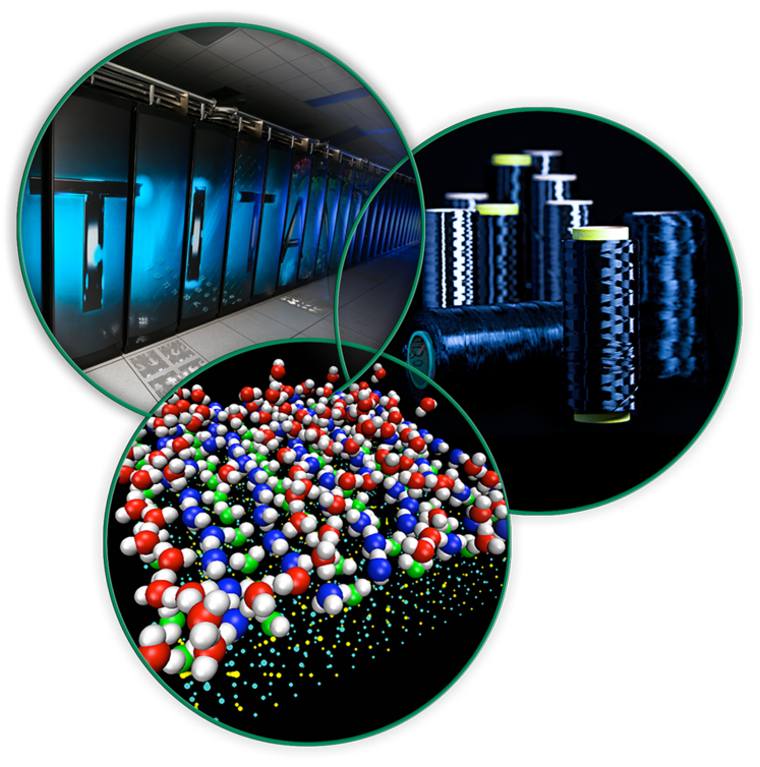
\includegraphics[width=1.5in]{ORNL_Balls.pdf}}

\defbeamertemplate{footline}{titlefoot}{
    \vspace{-0.5cm}
    \hspace*{0.25cm}
    
\includegraphics[width=2cm]{doe_logo}
    \hfill
    
\includegraphics[width=3.25cm]{WordMarkLeaf}
    \hspace*{0.5cm}
}

\setbeamertemplate{title page}
{
  \begin{tabular}{cr}
    \begin{minipage}{4.7cm}
      {\bf \Large\textcolor{MSUgreen}{\inserttitle}}\\

      \vspace{2\baselineskip}
      \insertauthor\\

      \insertinstitute\\

      \insertdate
    \end{minipage}
    &
    \begin{minipage}{5cm}
      \raggedright
      \vspace{-0.75cm}
      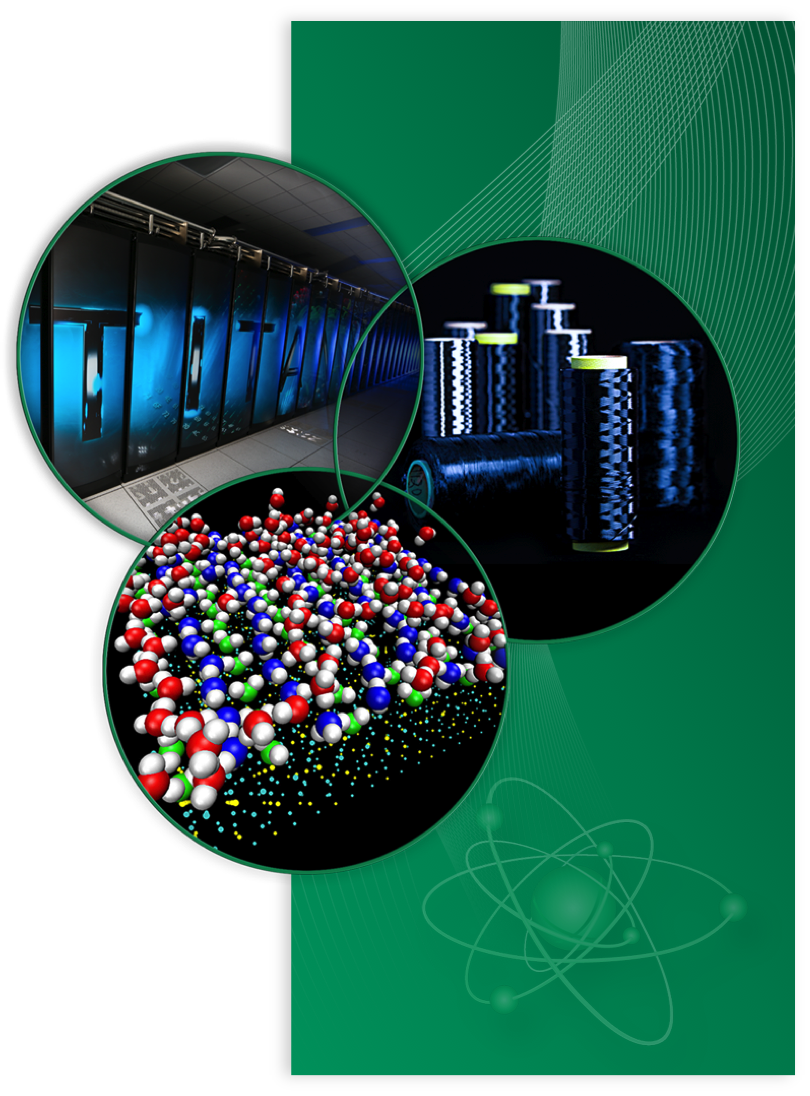
\includegraphics[height=9.8cm]{combined_background}
    \end{minipage}
  \end{tabular}
}

%%---------------------------------------------------------------------------%%
\begin{document}

%%---------------------------------------------------------------------------%%

{
\setbeamertemplate{logo}{}
\setbeamertemplate{footline}[titlefoot]
\begin{frame}
\titlepage
\end{frame}
}

%%---------------------------------------------------------------------------%%
\begin{frame}{Motivation}
  \vfill
\begin{itemize}
  \item As we move towards exascale computing, the rate of errors is expected
  to increase dramatically
  \vfil
  \begin{itemize}
    \item The probability that a compute node will fail during the course
      of a large scale calculation may be near 1
  \end{itemize}
  \vfill
  \item Algorithms need to not only have increased concurrency/scalability
    but have the ability to recover from hardware faults
\end{itemize}
  \vfill
\end{frame}
%%---------------------------------------------------------------------------%%
\begin{frame}{Towards Exascale Concurrency and Resiliency}
  \begin{itemize}
    \item Two basic strategies:
      \vfill
      \begin{enumerate}
        \item State with current ``state of the art'' methods and make
          incremental modifications to improve scalability and fault
          tolerance
          \begin{itemize}
            \item Many efforts are heading in this direction, attempting
              to find additional concurrency to exploit
          \end{itemize}
        \vfill
        \item Start with methods having natural scalability and resiliency
          aspects and work at improving performance
          \begin{itemize}
            \item One possibility: Monte Carlo methods
          \end{itemize}
      \end{enumerate}
  \end{itemize}
  \vfill
\end{frame}
%%---------------------------------------------------------------------------%%
\begin{frame}{Monte Carlo for Linear Systems}
  \begin{itemize}
    \item Suppose we want to solve $\mathbf{Ax}=\mathbf{b}$
    \vfill
    \item If $\rho(\mathbf{I-A})<1$, we can write the solution using the
      Neumann series
      \begin{equation*}
        \mathbf{x} = \sum_{n=0}^{\infty} (\mathbf{I-A})^n \mathbf{b}
         = \sum_{n=0}^{\infty} \mathbf{H}^n \mathbf{b}
      \end{equation*}
      where $\mathbf{H} \equiv ( \mathbf{I-A} )$ is Richardson iteration matrix
    \vfill
    \item Traverse the Neumann series stochastically
  \end{itemize}
\end{frame}
%%---------------------------------------------------------------------------%%
\begin{frame}{Forward Monte Carlo}
\begin{itemize}
  \item Choose a row-stochastic matrix $\mathbf{P}$ and weight matrix
    $\mathbf{W}$ such that $\mathbf{H} = \mathbf{P} \circ \mathbf{W}$
  \item Typical choice (Monte Carlo Almost-Optimal):
    \begin{equation*}
      \mathbf{P}_{ij} = \frac{| \mathbf{H}_{ij}| }
      {\sum_{j=1}^{N} | \mathbf{H}_{ij} | }
    \end{equation*}
  \item To compute solution component $\mathbf{x}_i$:
    \begin{itemize}
      \item Start a history in state $i$ (with initial weight of 1)
      \item Transition to new state $j$ based probabilities determined by
        $\mathbf{P}_i$
      \item Modify history weight based on corresponding entry in
        $\mathbf{W}_{ij}$
      \item Add contribution to $\mathbf{x}_i$ based on current history weight
        and value of $\mathbf{b}_j$
    \end{itemize}
  \item A given random walk can only contribute to a single component of
    the solution vector
\end{itemize}
\end{frame}
%%---------------------------------------------------------------------------%%
\begin{frame}{Adjoint Monte Carlo}
\begin{itemize}
  \item Choose $\mathbf{P}$ and $\mathbf{W}$ such that
    $\mathbf{H}^{T} = \mathbf{P} \circ \mathbf{W}$
  \item Typical choice (Monte Carlo Almost-Optimal):
    \begin{equation*}
      \mathbf{P}_{ij} = \frac{| \mathbf{H}_{ji}| }
      {\sum_{i=1}^{N} | \mathbf{H}_{ji} |}
    \end{equation*}
  \item To estimate solution:
    \begin{itemize}
      \item Start a history in random state $i$ by sampling from distribution
        determined by $\mathbf{b}$
      \item Transition to new state $j$ based probabilities determined by
        $\mathbf{P}_i$
      \item Modify history weight based on corresponding entry in
        $\mathbf{W}_{ij}$
      \item Add contribution to $\mathbf{x}_j$ based on current history weight
    \end{itemize}
  \item A given random walk can contribute to many different components of
    the solution vector
\end{itemize}
\end{frame}
%%---------------------------------------------------------------------------%%
\begin{frame}{Example (Forward Monte Carlo)}
  \begin{itemize}
    \item Suppose
  \begin{equation*}
    \mathbf{A} = \begin{bmatrix}
      \phmin 1.0 & -0.2 & -0.6 \\
      -0.4 & \phmin 1.0 & -0.4 \\
      -0.1 & -0.4 & \phmin 1.0 \end{bmatrix} \to
    \mathbf{H} \equiv (\mathbf{I-A}) = \begin{bmatrix}
       0.0 &  0.2 &  0.6 \\
       0.4 &  0.0 &  0.4 \\
       0.1 &  0.4 &  0.0 \end{bmatrix}
  \end{equation*}
    then
  \begin{equation*}
    \mathbf{P} = \begin{bmatrix}
       0.0 & 0.25 & 0.75 \\
       0.5 &  0.0 & 0.5 \\
       0.2 &  0.8 & 0.0 \end{bmatrix}, \quad
    \mathbf{W} = \begin{bmatrix}
       0.0 &  0.8 &  0.8 \\
       0.8 &  0.0 &  0.8 \\
       0.5 &  0.5 &  0.0 \end{bmatrix}
  \end{equation*}
    \vfill
    \item If a history is started in state $3$, there is a $20\%$ chance of
      it transitioning to state $1$ and an $80\%$ chance of moving to state
      $2$
  \end{itemize}
\end{frame}
%%---------------------------------------------------------------------------%%
\begin{frame}{Solving Heat Equation: Forward Method}

  \begin{figure}[h!]
    \begin{center}
      \includegraphics<1>[width=4in]{direct_1.png}
      \includegraphics<2>[width=4in]{direct_10.png}
      \includegraphics<3>[width=4in]{direct_100.png}
      \includegraphics<4>[width=4in]{direct_1000.png}
    \end{center}
    \caption{
      \only<1>{\textbf{Forward solution.}
        \textit{\sn{2.5}{3} total histories.} }
      \only<2>{\textbf{Forward solution.}
        \textit{\sn{2.5}{4} total histories.} }
      \only<3>{\textbf{Forward solution.}
        \textit{\sn{2.5}{5} total histories.} }
      \only<4>{\textbf{Forward solution.}
        \textit{\sn{2.5}{6} total histories.} }
    }
  \end{figure}

\end{frame}

%%---------------------------------------------------------------------------%%
\begin{frame}{Solving Heat Equation: Adjoint Method}

  \begin{figure}[h!]
    \begin{center}
      \includegraphics<1>[width=4in]{adjoint_1.png}
      \includegraphics<2>[width=4in]{adjoint_10.png}
      \includegraphics<3>[width=4in]{adjoint_100.png}
      \includegraphics<4>[width=4in]{adjoint_1000.png}
      \includegraphics<5>[width=4in]{adjoint_10000.png}
      \includegraphics<6>[width=4in]{adjoint_100000.png}
      \includegraphics<7>[width=4in]{adjoint_1000000.png}
      \includegraphics<8>[width=4in]{adjoint_10000000.png}
    \end{center}
    \caption{
      \only<1>{\textbf{Adjoint solution.}
        \textit{\sn{1}{0} total histories.} }
      \only<2>{\textbf{Adjoint solution.}
        \textit{\sn{1}{1} total histories.} }
      \only<3>{\textbf{Adjoint solution.}
        \textit{\sn{1}{2} total histories.} }
      \only<4>{\textbf{Adjoint solution.}
        \textit{\sn{1}{3} total histories.} }
      \only<5>{\textbf{Adjoint solution.}
        \textit{\sn{1}{4} total histories.} }
      \only<6>{\textbf{Adjoint solution.}
        \textit{\sn{1}{5} total histories.} }
      \only<7>{\textbf{Adjoint solution.}
        \textit{\sn{1}{6} total histories.} }
      \only<8>{\textbf{Adjoint solution.}
        \textit{\sn{1}{7} total histories.} }
    }
  \end{figure}
\end{frame}
%%---------------------------------------------------------------------------%%
\begin{frame}{Limitations of Monte Carlo}
\begin{itemize}
  \item Solving linear systems of equations with ``pure'' Monte Carlo methods
    is generally intractable
    \begin{itemize}
      \item Central limit theorem is barrier to accurate solutions
    \end{itemize}
\end{itemize}
\begin{figure}
  \centering
  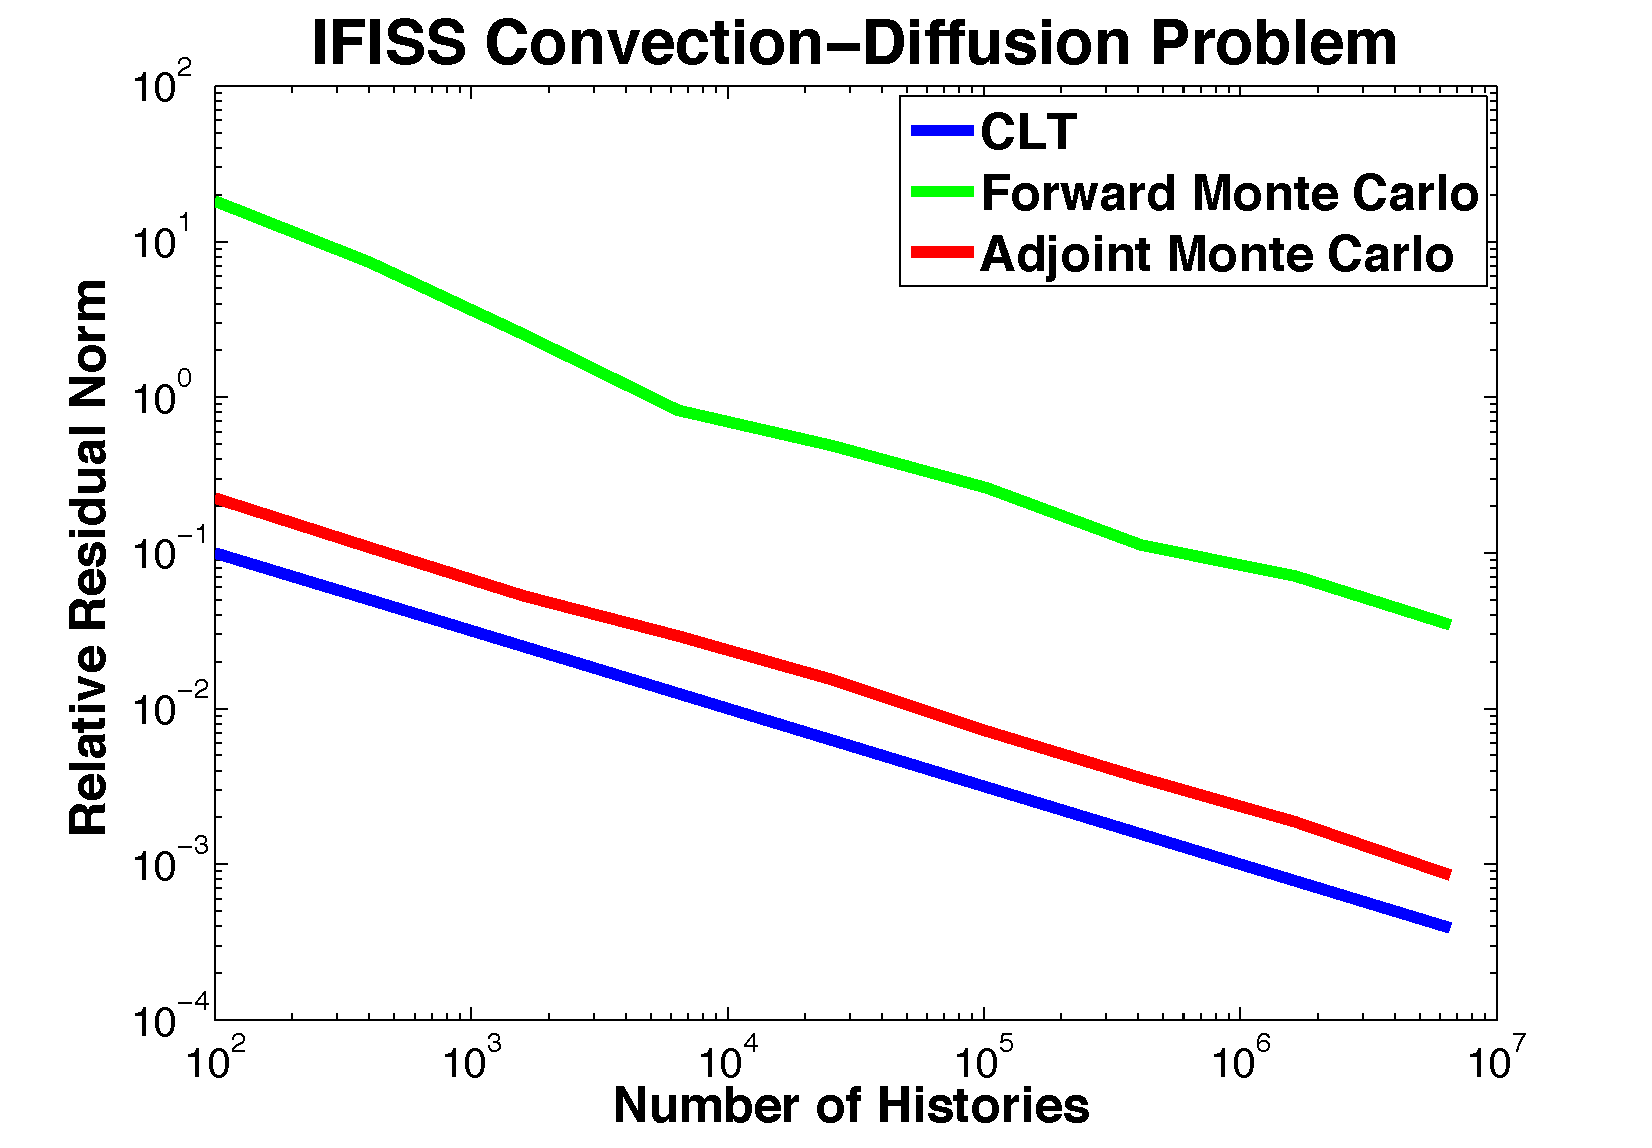
\includegraphics[width=3.5in]{Ifiss_ConvDiff}
\end{figure}
\end{frame}
%%---------------------------------------------------------------------------%%
\begin{frame}{Beyond the Central Limit Theorem}
  \begin{itemize}
    \item Instead of directly solving $\mathbf{Ax}=\mathbf{b}$ with Monte
      Carlo, apply Monte Carlo to residual equation
      $\mathbf{A}\delta = \mathbf{r}$
    \vfill
    \item Preconditioned Richardson iteration using Monte carlo as
      preconditioner:
      \begin{align*}
        \mathbf{r}^{k} &= \mathbf{b} - \mathbf{Ax}^{k} \\
        \hat{\mathbf{A}} \mathbf{\delta} &= \mathbf{r}^{k} \\
        \mathbf{x}^{k+1} &= \mathbf{x}^k + \delta
      \end{align*}
    \vfill
    \item This is the sequential Monte Carlo method devised by Halton
  \end{itemize}
\end{frame}
%%---------------------------------------------------------------------------%%
\begin{frame}{Further Beyond the Central Limit Theorem}
  \begin{itemize}
    \item Combine with Richardson iteration as a ``smoother'' in between
      Monte Carlo steps:
      \begin{align*}
        \mathbf{r}^k &= \mathbf{b} - \mathbf{Ax}^k \\
        \mathbf{x}^{k+1/2} &= \mathbf{x}^k + \mathbf{r}^k \\
        \mathbf{r}^{k+1/2} &= \mathbf{b} - \mathbf{Ax}^{k+1/2} \\
        \hat{\mathbf{A}} \mathbf{\delta} &= \mathbf{r}^{k+1/2} \\
        \mathbf{x}^{k+1} &= \mathbf{x}^{k+1/2} + \delta
      \end{align*}
    \vfill
    \item We call this algorithm Monte Carlo Synthetic Acceleration (MCSA)
  \end{itemize}
\end{frame}
%%---------------------------------------------------------------------------%%
\begin{frame}{Algorithm Comparison}
  \begin{figure}
    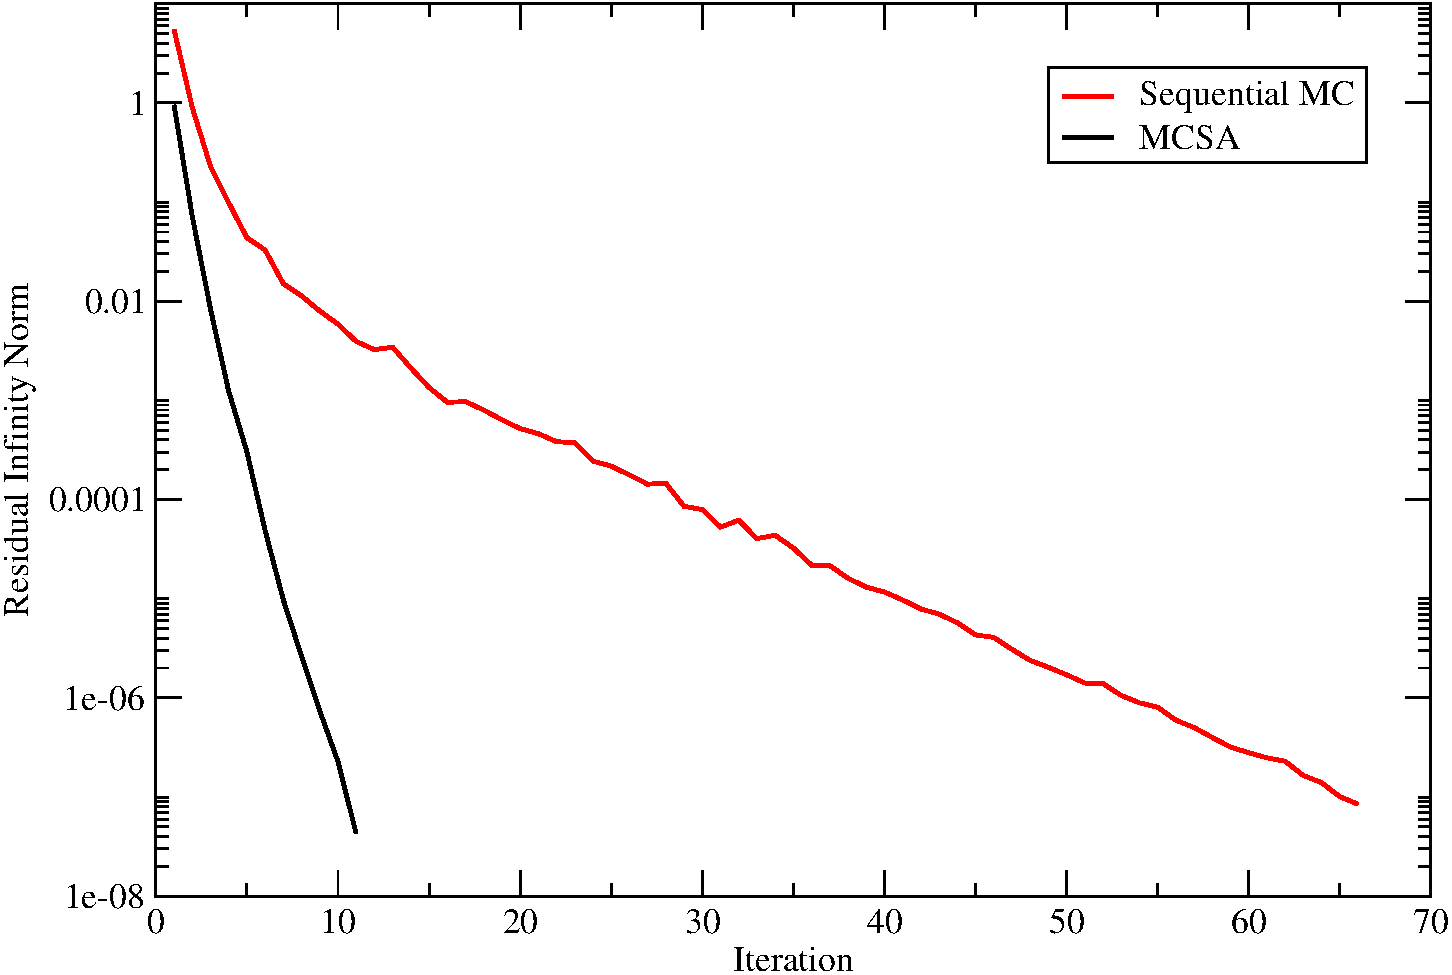
\includegraphics[width=3.5in]{seq_conv_100}
  \end{figure}
\end{frame}
%%---------------------------------------------------------------------------%%
\begin{frame}{Recent Success}
\begin{itemize}
  \item T. Evans, S. Mosher, S. Slattery, S. Hamilton, ``A Monte Carlo
    synthetic-acceleration method for solving the thermal radiation diffusion
    equation,'' Journal of Computational Physics \textbf{258},
    pp.~338--358 (2014).
  \item Applied MCSA to time-dependent thermal radiation diffusion equation
\end{itemize}
\begin{table}
  \centering
  \begin{tabular}{cccc}
    \toprule
    \multirow{2}{*}{\bfseries Solver} &
    \bfseries Total &
    \bfseries Relative Time &
    \bfseries Relative Total \\
    & \bfseries Iterations &
    \bfseries Per Iteration &
    \bfseries Time \\
    \midrule
    CG (ML) & 12150 & 74.7 & 2.7 \\
    GMRES (ILU) & 40294 & 103.0 & 9.2 \\
    MCSA & 98863 & 1.0 & 1.0 \\
    \bottomrule
  \end{tabular}
\end{table}
\end{frame}
%%---------------------------------------------------------------------------%%
\begin{frame}{Path to Harder Problems}
  \begin{itemize}
    \item Experience with radiation diffusion suggests that for problems
      where spectral radius is low ($\lesssim 0.8$),
      MCSA can be competitive with leading methods
      \begin{itemize}
        \item Very low cost per iteration to approximate Neumann series
      \end{itemize}
    \vfill
    \item What about more challenging problems?
      \begin{itemize}
        \item Neumann series converges more slowly, so histories last longer
        \item More histories may be required
        \item What if Neumann series is not convergent?
      \end{itemize}
  \end{itemize}
\end{frame}
%%---------------------------------------------------------------------------%%
\begin{frame}{Stopping Criteria -- Weight Cutoff}
  \begin{itemize}
    \item Histories are usually terminated when the relative weight drops
      below a specified cutoff (i.e. $\frac{w}{w_0} < \tau$)
    \vfill
    \item Adjoint MCSA on JPWH\_991 matrix with diagonal preconditioning
      ($\rho ( \mathbf{I-D^{-1}A} ) \approx 0.98$):
  \end{itemize}
\begin{figure}
  \centering
  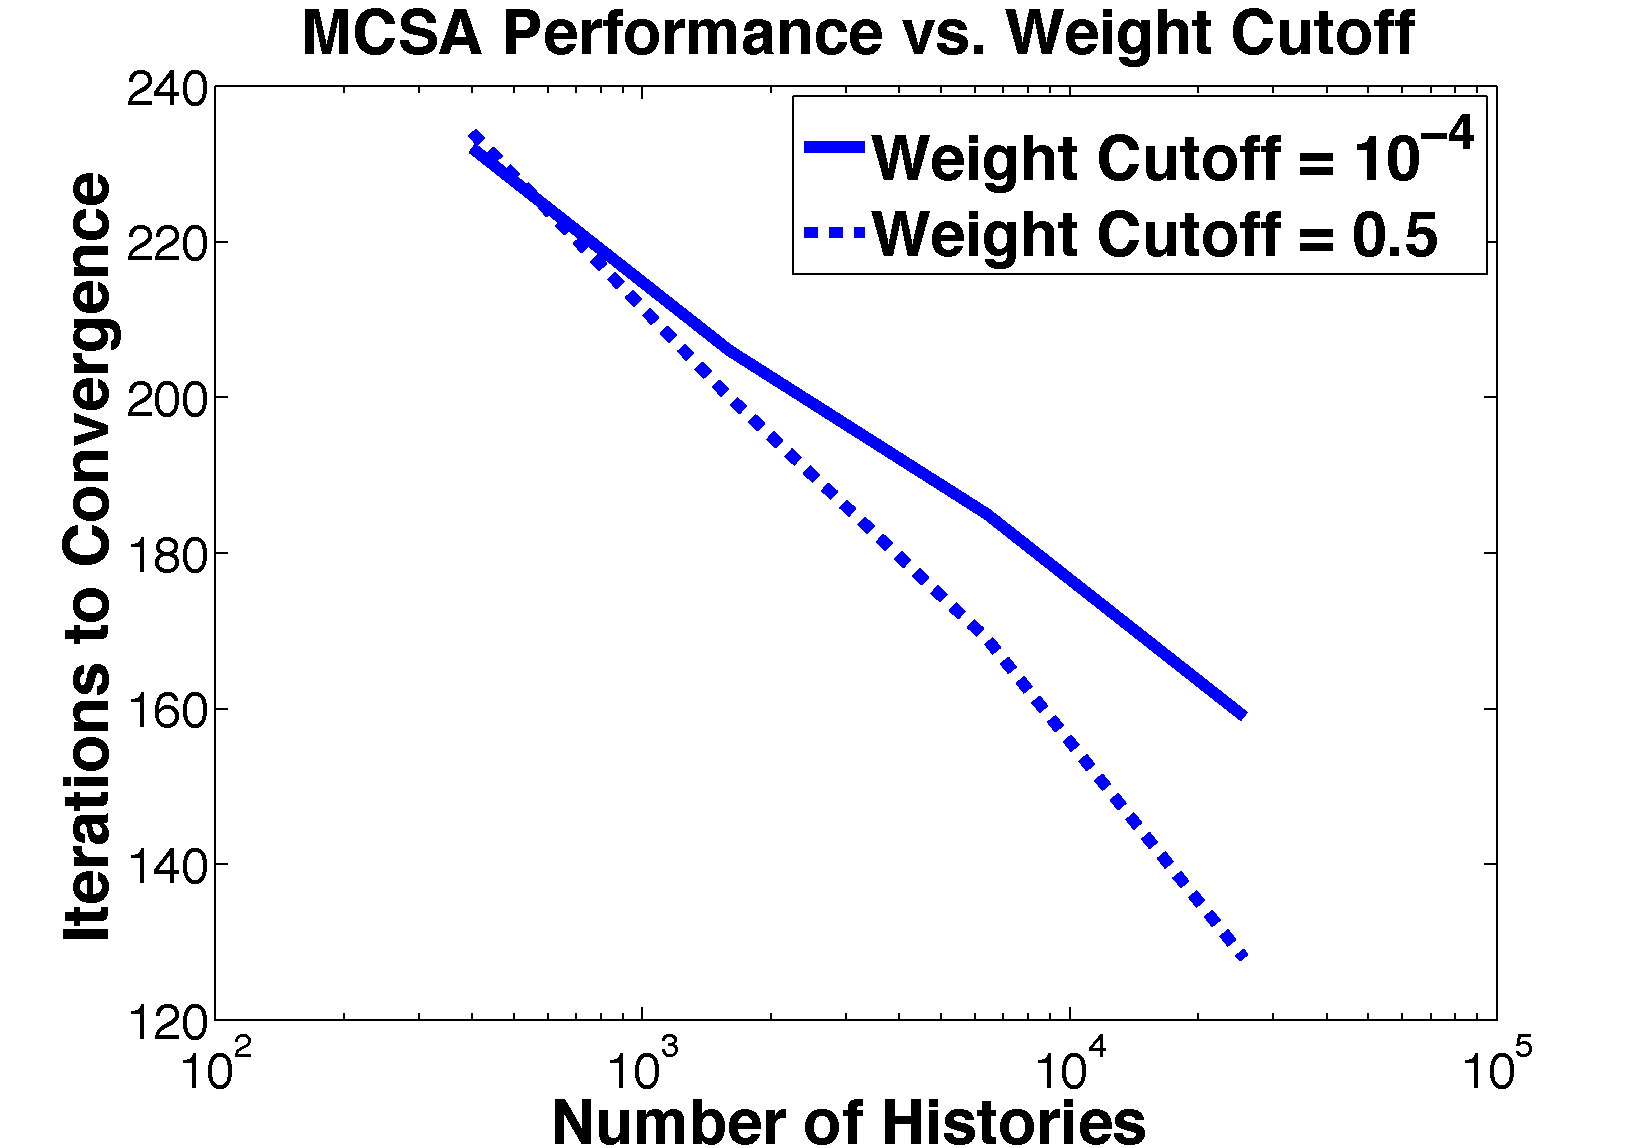
\includegraphics[width=2.5in]{WtCutoff}
\end{figure}
\end{frame}
%%---------------------------------------------------------------------------%%
\begin{frame}{Stopping Criteria -- History Length Cutoff}
  \begin{itemize}
    \item Somewhat counterintuitive result: using larger weight cutoff often
      results in better MCSA convergence
      \begin{itemize}
        \item A good approximation to a few terms in the Neumann series
          performs better than a statistically noisy approximation to
          full series
      \end{itemize}
    \vfill
    \item If statistical performance is better for large weight cutoff,
      what happens if we simply terminate histories after prescribed number
      of steps
  \end{itemize}
\end{frame}
%%---------------------------------------------------------------------------%%
\begin{frame}{Weight vs. History Length Cutoff}
\begin{figure}
  \centering
  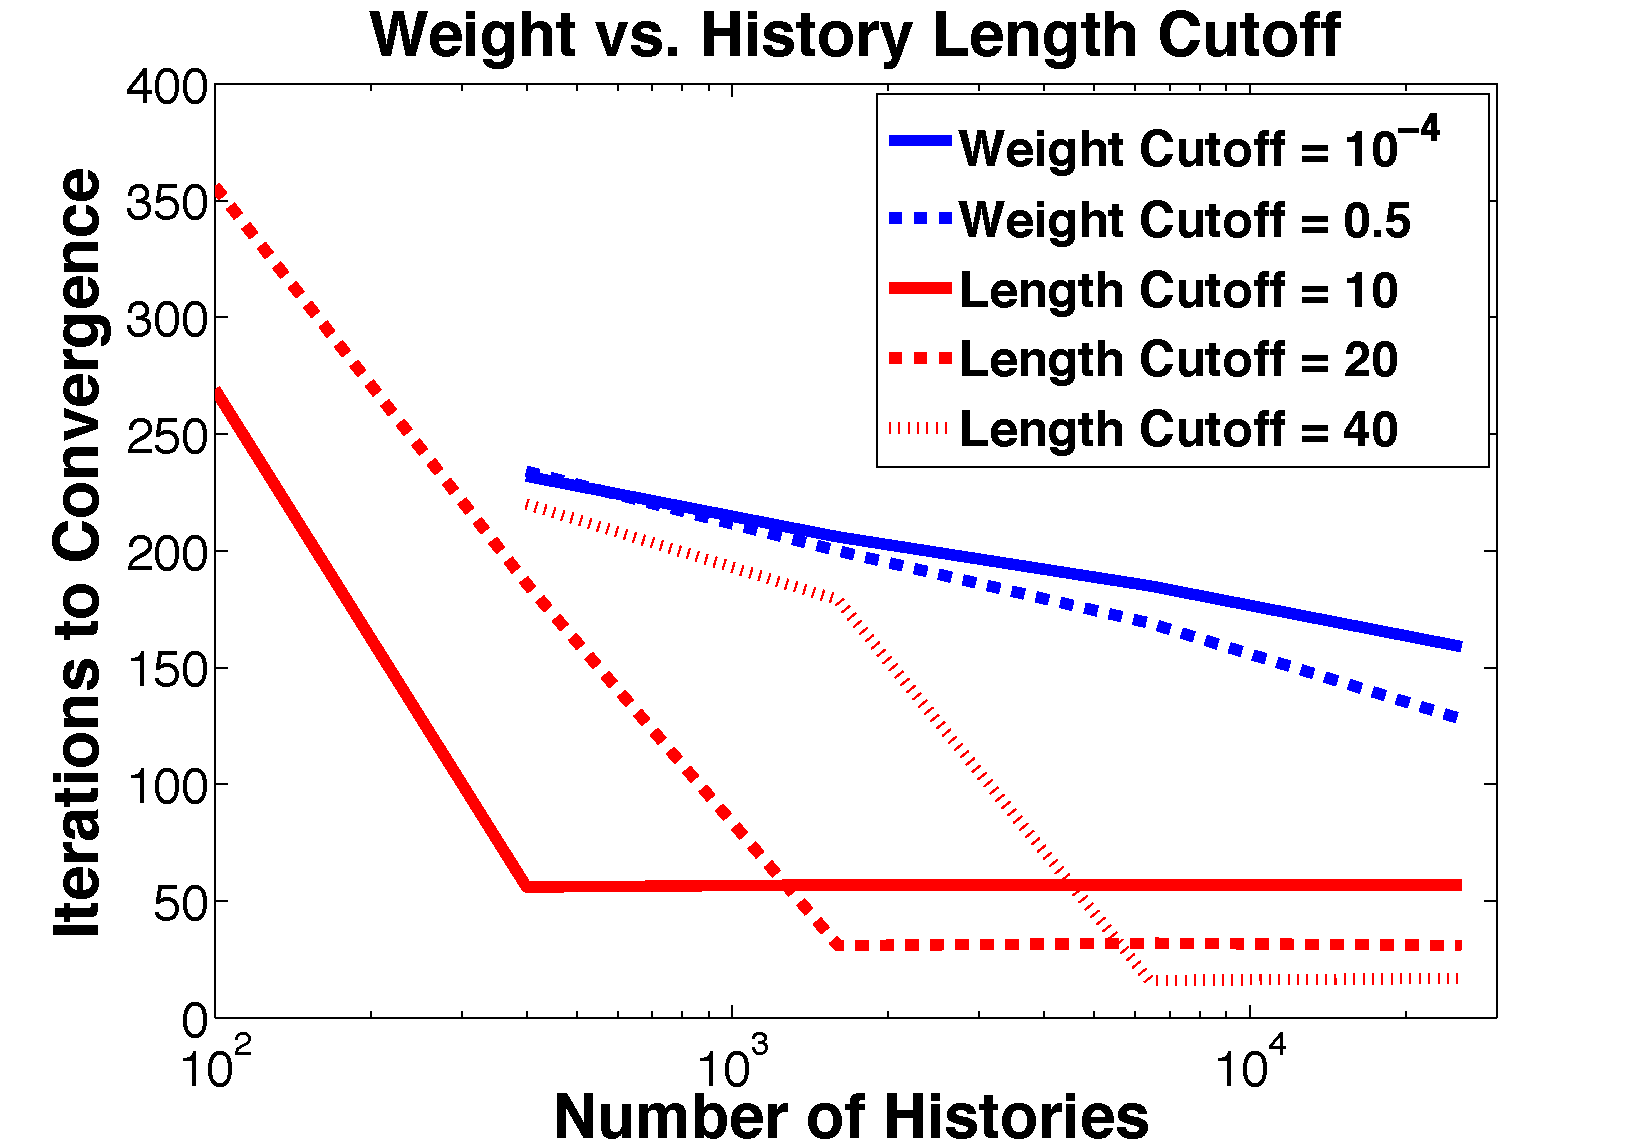
\includegraphics[width=3in]{WtVsLength}
\end{figure}
\begin{itemize}
  \item Unlike weight cutoff, history length cutoff ``saturates'' at some
    number of histories -- fixed length Neumann series has been perfectly
    reproduced
  \item Saturation point is higher for longer history lengths
\end{itemize}
\end{frame}
%%---------------------------------------------------------------------------%%
\begin{frame}{Monte Carlo as Approximate Polynomial Preconditioning}
  \begin{itemize}
    \item Using history length cutoff, Monte Carlo process is approximating
      a fixed length Neumann series polynomial
    \vfill
    \item As number of histories grows, iteration count becomes identical to
      using ``true'' polynomial
    \vfill
    \item Why limit ourselves to the Neumann series polynomial?
      \begin{itemize}
        \item Chebyshev or GMRES polynomials are viable alternatives
      \end{itemize}
  \end{itemize}
\end{frame}
%%---------------------------------------------------------------------------%%
\begin{frame}{Neumann Series Polynomial}
\begin{table}
\caption{Adjoint MCSA with Neumann Polynomial, $1000 \times 1000$ Shifted Laplacian Matrix.
Values are MCSA iteration counts (timing in milliseconds)
\label{tab:lap_adjoint_neumann}}
\centering
\begin{tabular}{cccc}
\toprule
Histories per & \multicolumn{3}{c}{Polynomial Order} \\
\cmidrule(lr){2-4}
Iteration & 2 & 4 & 6 \\
\midrule
250 &  775(100) & 651(96) & 664(110) \\
500 &  725(122) & 502(104) & 394(95) \\
1000 & 707(174) & 482(179) & 366(144) \\
2000 & 703(280) & 471(259) & 356(251) \\
4000 & 698(494) & 467(497) & 350(458) \\
8000 & 697(923) & 464(905) & 350(873) \\
16000 & 695(1796) & 462(1768) & 347(1711) \\
\bottomrule
\end{tabular}
\end{table}
\end{frame}
%%---------------------------------------------------------------------------%%
\begin{frame}{Chebyshev Polynomial}
\begin{table}
\caption{Adjoint MCSA with Chebyshev Polynomial, $1000 \times 1000$ Shifted Laplacian Matrix.
Values are MCSA iteration counts (timing in milliseconds)
\label{tab:lap_adjoint_cheby}}
\centering
\begin{tabular}{cccc}
\toprule
Histories per & \multicolumn{3}{c}{Polynomial Order} \\
\cmidrule(lr){2-4}
Iteration & 1 & 2 & 3 \\
\midrule
250 & - & - & - \\
500 & - & - & - \\
1000 & - & - & - \\
2000 & - & 328(134) & - \\
4000 & - & 296(210) & - \\
8000 & - & 288(380) & 262(423) \\
16000 & 1132(1866) & 283(721) & 175(550) \\
\bottomrule
\end{tabular}
\end{table}
\end{frame}
%%---------------------------------------------------------------------------%%
\begin{frame}{GMRES Polynomial}
\begin{table}
\caption{Adjoint MCSA with GMRES Polynomial, $1000 \times 1000$ Shifted Laplacian Matrix.
Values are MCSA iteration counts (timing in milliseconds)
\label{tab:lap_adjoint_gmres}}
\centering
\begin{tabular}{cccc}
\toprule
Histories per & \multicolumn{3}{c}{Polynomial Order} \\
\cmidrule(lr){2-4}
Iteration & 2 & 4 & 6 \\
\midrule
250 &  2572(337) & - & - \\
500 &  616(105)  & - & - \\
1000 & 566(142)  &  - & - \\
2000 & 557(222)  &  - & - \\
4000 & 554(412)  &  203(236) & - \\
8000 & 549(731)  &  184(423) & - \\
16000 & 548(1426) & 247(965) & 146(744) \\
\bottomrule
\end{tabular}
\end{table}

\end{frame}
%%---------------------------------------------------------------------------%%
\begin{frame}{Polynomial Methods -- Summary}
  \begin{itemize}
    \item Using history length cutoff rather than weight cutoff can lead to
      large reductions in iteration counts
    \vfill
    \item Significant reduction in iteration counts are possible using
      alternate polynomials, but generally outweighed by increase in number
      of histories required
      \begin{itemize}
        \item May be very beneficial from resiliency and parallel efficiency
          standpoints
        \item Will be re-evaluated in future efforts
      \end{itemize}
  \end{itemize}
\end{frame}
%%---------------------------------------------------------------------------%%
\begin{frame}{Preconditioning}
  \begin{itemize}
    \item If a non-trivial preconditioner is used, the Monte Carlo problem
      must be formed based on preconditioned iteration matrix,
      $\mathbf{H} = \mathbf{I-M^{-1}A}$
    \vfill
    \item Requires explicit construction of preconditioned matrix
      \begin{itemize}
        \item This has generally limited preconditioner selection to diagonal,
          block diagonal, sparse approximate inverse approaches
      \end{itemize}
    \vfill
    \item Sparsity in $\mathbf{A}$, $\mathbf{M}$, does not imply sparsity
      in $\mathbf{M^{-1}A}$
    \vfill
    \item Need to investigate preconditoning strategies that lead to sparse
      preconditioned systems (Michele/Max)
  \end{itemize}
\end{frame}
%%---------------------------------------------------------------------------%%
\begin{frame}[fragile]{Multiple-Set Overlapping-Domain Decomposition}

  \vspace{-1cm}
  \begin{columns}

    \begin{column}{0.52\textwidth}

      \begin{figure}[t!]
        \begin{center}
          \scalebox{0.275}{ \input{msod_construction.pdftex_t} }
        \end{center}
        \caption{\small MSOD construction.}
      \end{figure}

    \end{column}

    \begin{column}{0.48\textwidth}

      \begin{figure}[t!]
        \begin{center}
          \scalebox{0.2}{ \input{msod_tally.pdftex_t} }
        \end{center}
        \caption{\small MSOD tally reduction.}
      \end{figure}

      \begin{itemize}
        {\small
        \item Multiple sets replicate the domain
        \item Domains overlap within a set
        \item Each set contains the full domain
        }
      \end{itemize}

    \end{column}

  \end{columns}

%  \let\thefootnote\relax\footnote{\tiny{Wagner et. al., "Hybrid and
%      parallel domain-decomposition methods development to enable
%      Monte Carlo for reactor analysis", Joint International
%      Conference on Supercomputing in Nuclear Applications and Monte
%      Carlo (SNA+MC 2010), 2010.}}

\end{frame}

%%---------------------------------------------------------------------------%%
\begin{frame}{Alternative Parallelism -- Additive Schwarz}
  \begin{itemize}
    \item Instead of performing Monte Carlo on full problem, another
      possibility is to apply Monte Carlo as an additive Schwarz approach
    \vfill
    \item Decompose problem into (possibly overlapping) domains
    \vfill
    \item Perform Monte Carlo on individual subdomains
      \begin{itemize}
        \item No communication costs in Monte Carlo problem!
      \end{itemize}
    \vfill
    \item With domain decomposed Monte Carlo, iteration counts are effectively
      independent of the number of processors
    \vfill
    \item In an additive Schwarz approach, the preconditioner will become
      less effective as processor counts grow -- algorithmic scalability
      may be an issue
  \end{itemize}
\end{frame}
%%---------------------------------------------------------------------------%%
\begin{frame}{More Parallelism -- Threading}
  \begin{itemize}
    \item Within a Monte Carlo solve, every history is independent of other
      histories -- great potential for highly concurrent hardware
      (GPU, Xeon Phi)
    \vfill
    \item Early experiments using the Trilinos Kokkos library show promising
      performance for multicore CPUs
    \vfill
    \item Will be taking part in OLCF ``Hackathon'' in late October to begin
      implementing computation kernels in OpenACC to allow GPU capability
  \end{itemize}
\end{frame}
%%---------------------------------------------------------------------------%%
\begin{frame}{Application -- Nuclear Reactor Analysis}
  \begin{itemize}
    \item The simplified $P_N$ ($SP_N$) equations are an approximation
      to the Boltzmann neutron transport equation used to simulate nuclear
      reactors
      \begin{itemize}
        \item We are interested in solving generalized eigenvalue problem,
          for this study we use Arnoldi as the eigensolver and compare
          different methods for solving linear systems
      \end{itemize}
    \vfill
    \item Test problem -- $3 \times 3$ array of fuel assemblies with
      control rod in center location
      \begin{itemize}
        \item 23 energy groups, 2 angular moments, 25M degrees of freedom
        \item 1000 computational cores
      \end{itemize}
  \end{itemize}
\end{frame}
%%---------------------------------------------------------------------------%%
\begin{frame}{SPN Solution}
  \begin{figure}
    \centering
    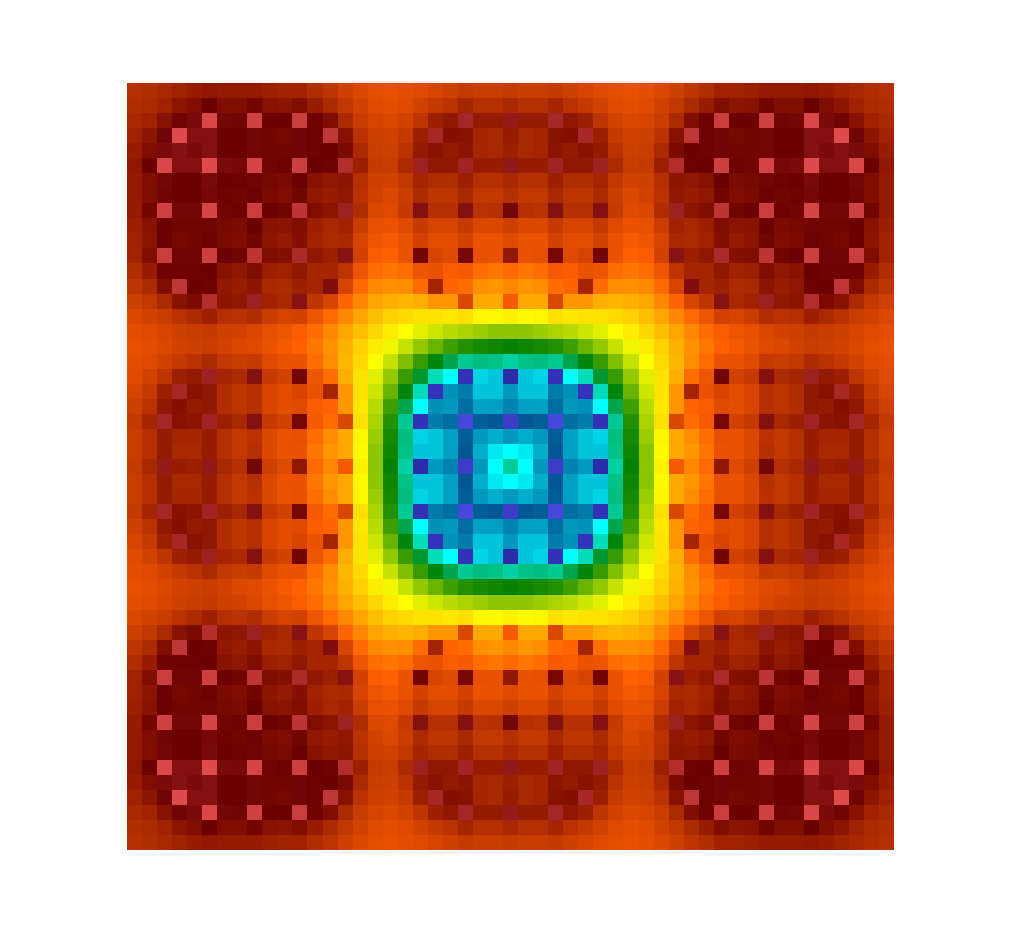
\includegraphics[width=3in]{prob4}
  \end{figure}
\end{frame}
%%---------------------------------------------------------------------------%%
\begin{frame}{SPN Results}
\begin{table}
\centering
\begin{tabular}{cccc}
\toprule
%Method & Total GMRES Iterations & Setup Time (s) & Solve Time (s) \\
\multirow{2}{*}{\bfseries Method} &
\bfseries Total GMRES & \bfseries Setup & \bfseries Solve \\
& \bfseries Iteration & \bfseries Time (s) & \bfseries Time (s) \\
\midrule
GMRES-ILUT      & 1675 & 0.7  & 18.4 \\
GMRES-AMG       & 626  & 0.7  & 46.0 \\
GMRES-MGE       & 498  & 1.5  & 33.7 \\
Richardson-AINV & 5208 & 20.6 & 52.0 \\
MCSA-AINV       & 1268 & 25.5 & 46.6 \\
\bottomrule
\end{tabular}
\end{table}
\begin{itemize}
  \item ILUT preconditioning is winner here, but known to have issues
    with parallel scaling on large core counts
  \item Solve times for MCSA are competitive, but setup times are very large
    due to types of preconditioning necessary
\end{itemize}
\end{frame}
%%---------------------------------------------------------------------------%%
\begin{frame}{Additional Thoughts}
  \begin{itemize}
    \item Our current implementations rely on performing fixed number of
      histories per Monte Carlo solve
      \begin{itemize}
        \item How can we dynamically select/adapt the number of histories
          that should be performed?  Use variance-based stopping criteria?
      \end{itemize}
    \vfill
    \item The ``almost optimal'' selection of the probability and weight
      matrices is arbitrary (as long as
      $\mathbf{H}/\mathbf{H}^T=\mathbf{P} \circ \mathbf{W}$)
      \begin{itemize}
        \item If $\mathbf{P}$ is taken to have a uniform distribution within
          each row, then sampling from the distribution can be done in
          constant (rather than logarithmic) time
      \end{itemize}
    \vfill
    \item Anderson acceleration of MCSA (Tim Kelly @ NCSU)
  \end{itemize}
\end{frame}
%%---------------------------------------------------------------------------%%
\begin{frame}{Conclusions}
  \begin{itemize}
    \item Monte Carlo methods offer great potential for both resilient and
      highly parallel solvers
    \vfill
    \item For certain classes of problems, Monte Carlo methods can be
      competitive with leading modern solvers
    \vfill
    \item Extending methods to broader problem areas is significant challenge
      and an attractive area for continued research
  \end{itemize}
\end{frame}

%%---------------------------------------------------------------------------%%
\end{document}
%%---------------------------------------------------------------------------%%

%%---------------------------------------------------------------------------%%
%% end of pres.tex
%%---------------------------------------------------------------------------%%
